\documentclass[a4paper, 12pt]{article}
\usepackage[utf8]{inputenc}

\title{A.I. Course Assignment}
\author{Vlad Vasilescu - CEN 2.3B}
\date{Problem 3}

\usepackage{natbib}
\usepackage{graphicx}
\usepackage{indentfirst}
\usepackage{hyperref}

\begin{document}

\maketitle

\section*{Determining the correct problem:}
For finding the correct problem I wrote a simple function in python which takes a string and hashes it
in the specified way. The function can be found in the file hash\_name.py

\section*{Problem statement:}
A basic wooden railway set contains the pieces shown below. The task is to connect these pieces into a railway
that has no overlapping tracks and no loose ends where a train could run off onto the floor. \par
\begin{itemize}
    \item Suppose that the pieces fit together exactly with no slack. Give a precise formulation of the task
    as a search problem.
    \item Identify a suitable search algorithm for this task and explain your choice.
\end{itemize}

\section*{Formulation as a search problem:}
For the initial state we take an empty track where any piece can be placed on the starting position. The track
can be represented as graph where each piece is a node. In order to avoid overlapping we also have to keep track
of the positon of each piece (node) and whenever we add a new one make sure that positon is empty. \par
A new piece can be added to any open path of an already existing piece. \par
Instead of comparing the state to a goal we check that all pieces are used and that there is no path left open.

\section*{Problem implementation:}
I've chosen to represent the track pieces as lines which are easier to draw and connect and have similar
properties to the pieces. \par
For the straight piece it's just a straight line, for the curved piece it's a
45 degree angled line and for the other two pieces its a combination of straight plus angled line. \par
The points at the ends of the lines can be of two types: "male" and "female". Only two points of oposite
types can connect to each other. \par
The pieces can be found in the track\_pieces.json file. Each piece is made out of a list of so called
"edges" which represent the connections. Each one of those points has a position relative to the origin of the piece,
an angle and a type. The piece is made up by drawing lines between every of these "edges" where the types differ.

\section*{Search algorithm:}
For search algorithm I've used Best-first search. \par
The heuristic used is the sum of the distances between "edge" left open to the origin and their total number.

\section*{Notes:}
Unfortunetly, even with a simpler implementation the problem has too many possible paths with the given number of
pieces. The best case I managed to simulate was with only 8 of the curved pieces and 4 of the straight ones.
Perhaps better results can be achieved with a better heuristic and search algorithm. For the data set I've included
a roughly 3 second execution time can be expected on a midrange CPU (tested on a R5 2600 @ 3.9GHz).

\begin{figure}
    \centering
    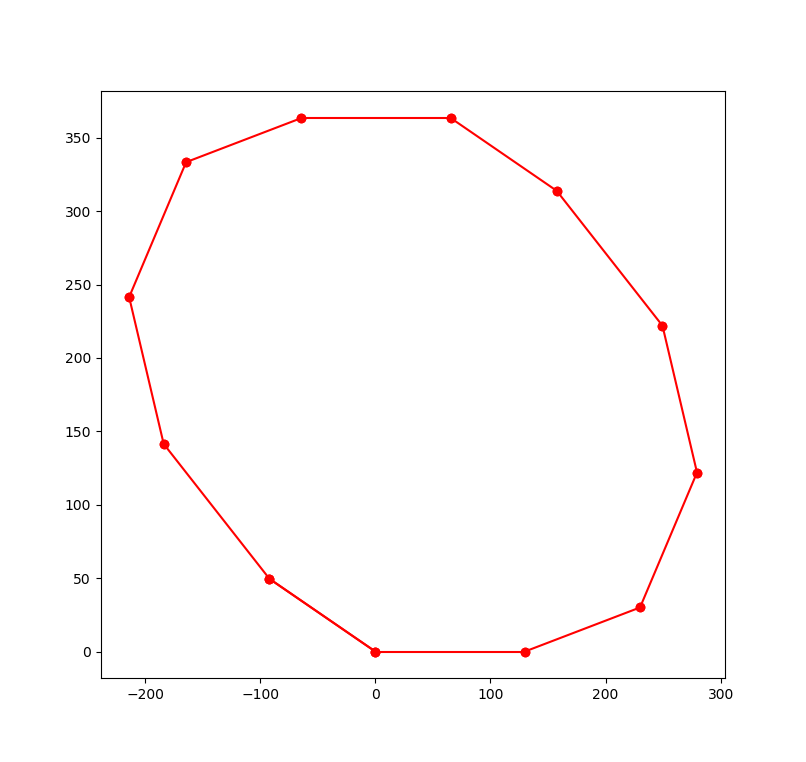
\includegraphics[scale=0.5]{Figure_2.png}
    \caption{8 curved and 4 straight pieces}
\end{figure}

\begin{figure}
    \centering
    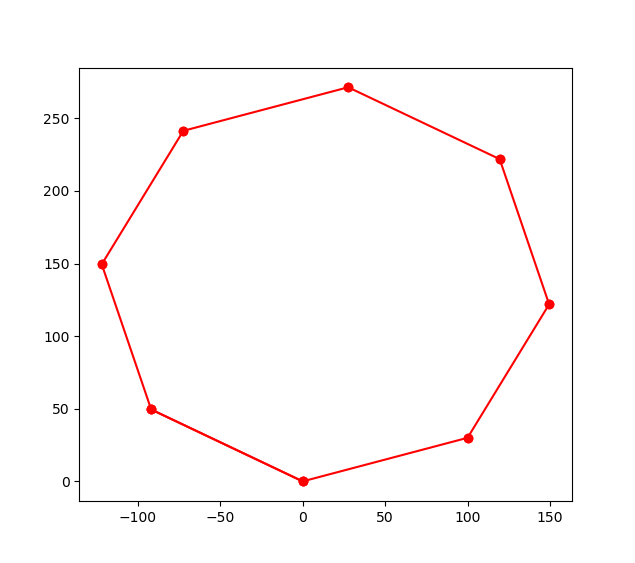
\includegraphics[scale=0.6]{Figure_1.png}
    \caption{8 curved pieces}
\end{figure}

\subsection*{Requirements:}
\begin{itemize}
    \item \href{https://matplotlib.org/users/installing.html}{Matplotlib}
\end{itemize}

\end{document}
